\documentclass{article}


\usepackage{arxiv}

\usepackage[utf8]{inputenc} % allow utf-8 input
\usepackage[T1]{fontenc}    % use 8-bit T1 fonts
\usepackage{hyperref}       % hyperlinks
\usepackage{url}            % simple URL typesetting
\usepackage{booktabs}       % professional-quality tables
\usepackage{amsfonts}       % blackboard math symbols
\usepackage{nicefrac}       % compact symbols for 1/2, etc.
\usepackage{microtype}      % microtypography
\usepackage{graphicx}
\usepackage{natbib}
\usepackage{doi}

\usepackage{amsmath}
\usepackage{nicematrix}
\usepackage{cleveref}
\usepackage{listings}
\usepackage{pgfplots}


\NiceMatrixOptions{cell-space-top-limit=5pt,cell-space-bottom-limit=5pt,columns-width=20pt}

\crefname{lstlisting}{listing}{listings}
\Crefname{lstlisting}{Listing}{Listings}


% Listing options
\definecolor{codegreen}{rgb}{0,0.6,0}
\definecolor{codegray}{rgb}{0.5,0.5,0.5}
\definecolor{codepurple}{rgb}{0.58,0,0.82}
\definecolor{backcolour}{rgb}{0.95,0.95,0.92}

\lstdefinestyle{python_style}{
    backgroundcolor=\color{backcolour},
    commentstyle=\color{codegreen},
    keywordstyle=\color{magenta},
    numberstyle=\tiny\color{codegray},
    stringstyle=\color{codepurple},
    basicstyle=\ttfamily\footnotesize,
    breakatwhitespace=false,
    breaklines=true,
    captionpos=b,
    keepspaces=true,
    numbers=left,
    numbersep=5pt,
    showspaces=false,
    showstringspaces=false,
    showtabs=false,
    tabsize=2
}
\lstset{style=python_style}


\newcommand{\irow}[1]{% inline row vector
  {\begin{smallmatrix}(\,#1\,)\end{smallmatrix}}^T
}


\def\R{\mathbb{R}}
\def\xt{\tilde{x}}


\title{Linear programming project}

%\date{September 9, 1985}	% Here you can change the date presented in the paper title
\date{} 					% Or removing it

\author{
  \hspace{1mm}Dmitry Beresnev \\
	MS-DS1, Innopolis University\\
	\texttt{d.beresnev@innopolis.university} \\
	\And{}
  \hspace{1mm}Vsevolod Klyushev \\
	MS-DS1, Innopolis University\\
	\texttt{v.klyushev@innopolis.university}
}

\renewcommand{\undertitle}{\textbf{Group 2} Report for Optimization F24 course}
\renewcommand{\headeright}{}

\begin{document}
\maketitle


\section{Introduction}
Initial problem is formulated as following:
\begin{equation}\label{eq:init}
  \begin{aligned}
                 & \min\limits_{x' \in \R^p} {\| Ax'-y' \|}_1 \\
    \text{s.t. } & 0 \leq x' \leq 1
  \end{aligned}
\end{equation}
where $A \in \R^{m \times p}$ with $m \geq p$ --- message  encoding matrix,
$y'$ --- received encoded (noisy) message,
$x'$ --- encoded initial message to be find.

\section{Notations}

 {
  \renewcommand{\arraystretch}{1.5}
  \renewcommand{\tabcolsep}{10pt}
  \begin{table}[h]
    \centering
    \begin{tabular}{cc}
      \toprule
      \textbf{Notation}                          & \textbf{Meaning}                                     \\
      \midrule
      $e_i$                                      & unit vector with 1 at index $i$ and all other zeroes \\
      $1_n$                                      & vector of $n$ ones                                   \\
      $I_n$                                      & identity matrix of size $n \times n$                 \\
      $0_n$                                      & vector of $n$ zeroes                                 \\
      $0_{m \times n}$                           & zero matrix of size $m \times n$                     \\
      $x_i$ $\left( \text{or } {(Ax)}_i \right)$ & $i$-th component of vector $x$    (or $Ax$)          \\

      \bottomrule
    \end{tabular}
  \end{table}
 }


\section{Q1: Linear problem formulation}
Initial problem (\cref{eq:init}) is not linear as cost function
$ {\| Ax'-y' \|}_1 = \sum_{i=1}^{m} |{(Ax')}_i-y'_i|$, is not linear. However, this objective function is \textbf{piecewise linear convex} function. Therefore, each element $|{(Ax')}_i-y'_i| = \max({(Ax')}_i-y'_i, y'_i -{(Ax')}_i)$ can be substituted with new variable $z'$ with the following additional
constraints: $z_i \geq {(Ax')}_i-y'_i$ and $z_i \geq y'_i-{(Ax')}_i$.

So the following problem is \textbf{linear} and is equivalent to the initial one:
\begin{equation}\label{eq:linear}
  \begin{aligned}
                 & \min\limits_{x' \in \R^p, z \in \R^m} \sum_{i=1}^{m} z_i \\
    \text{s.t. } & x' \geq 0                                                \\
                 & x' \leq 1                                                \\
                 & z_i \geq {(Ax')}_i-y'_i, \ i = 1 \dots m                 \\
                 & z_i \geq y'_i-{(Ax')}_i, \ i = 1 \dots m                 \\
  \end{aligned}
\end{equation}

\section{Q2: Linear problem in standard form}

For the easier and more evident deviation of standard form of \Cref{eq:linear},
linear problem will be firstly rewritten in geometric form, and only then --- in standard. The obtained linear optimization problem in standard form will be equivalent to initial problem (\cref{eq:init}).

\subsection{Geometric form}\label{sec:geom}

The equivalent \textbf{geometric} form of \Cref{eq:linear} is
\begin{equation}\label{eq:geom}
  \begin{aligned}
                 & \min\limits_{z' \in \R^{p+m}} c^T z' \\
    \text{s.t. } &
    \begin{pNiceArray}{c:c}
      I_p  & 0_{p \times m}  \\
      \hdottedline
      -I_p  & 0_{p \times m}  \\
      \hdottedline
      -A & I_m \\
      \hdottedline
      A & I_m \\
      \CodeAfter
      \UnderBrace[yshift=1.5mm,color=blue]{last-1}{last-last}{A'}
    \end{pNiceArray}
    z' \geq
    \begin{pNiceMatrix}
      0_p  \\
      -1_p \\
      -y'  \\
      y'   \\
      \CodeAfter
      \UnderBrace[yshift=1.5mm,color=blue]{last-1}{last-last}{b'}
    \end{pNiceMatrix},
  \end{aligned}
  \vspace{20pt}
\end{equation}
where
$c = \sum_{i=p+1}^{p+m} e_i \in \R^{(p+m)}$,
$b' \in \R^{2p+2m}$ and
$A'\in \R^{(2p+2m) \times (p+m)}$.

The first $p$ components of $z'$ correspond to the components of $x'$, and the next $m$ components correspond to the components of $z$ from \Cref{eq:linear}. Rows and columns of $A'$ representation in \Cref{eq:geom} are separated in blocks for clarity: the vertical separation is for $x'$ and $z$ correspondingly, and the horizontal separations denote corresponding constraints from \Cref{eq:linear}.

\subsection{Standard form}\label{sec:std}

Note that $z' = {(x', z)}^T$ from \Cref{eq:geom} is already non-negative, because $x' \geq 0$ by problem definition and $z \geq 0 $ by construction\footnote{Intuitively, $z$ substitutes the absolute value, so is non-negative. Formally, from \Cref{eq:linear}, $z \geq t$ and $z \geq -t$ for some $t$. So if $t \geq 0$, then $z \geq t \geq 0$, and if $t \leq 0$ then $z \geq -t \geq 0$ }. Therefore, to convert \Cref{eq:geom} to standard form, only introduction of slack variables is needed to get rid of inequality sign. The equivalent \textbf{standard} form of \Cref{eq:geom} is
\begin{equation}\label{eq:std}
  \begin{aligned}
                 & \min\limits_{\xt \in \R^{2p+3m}} c^T \xt    \\
    \text{s.t. } &
    \begin{pNiceArray}{c:c:c}
      -I_p  & 0_{p \times m} & -S^{1,p}  \\
      \hdottedline
      -A & I_m & -S^{p+1,p+m} \\
      \hdottedline
      A & I_m & -S^{p+m+1,p+2m}\\
      \CodeAfter
      \UnderBrace[yshift=1.5mm,color=blue]{last-1}{last-last}{A'}
    \end{pNiceArray}
    z' =
    \begin{pNiceMatrix}
      -1_p \\
      -y'  \\
      y'   \\
      \CodeAfter
      \UnderBrace[yshift=1.5mm,color=blue]{last-1}{last-last}{b'}
    \end{pNiceMatrix}, \\
    \vspace{20pt}                                              \\
                 & \xt \geq 0,
  \end{aligned}
  \vspace{20pt}
\end{equation}
where
$c = \sum_{i=p+1}^{p+m} e_i \in \R^{(2p+3m)}$,
$b' \in \R^{p+2m}$,
$A'\in \R^{(p+2m) \times (2p+3m)}$, and
$S^{a,b}$ --- slack variable matrix of size $(b-a+1) \times (p+2m)$
with rows $S^{a,b}_i = e_{a+i-1}$, which represents necessary slack variables.

The first $p$ components of $\xt$ correspond to the components of $x'$, the next $m$ components correspond to the components of $z$ from \Cref{eq:linear} and the last $(p+2m)$ components correspond to slack variables $s$. Rows and columns of $A'$ representation in \Cref{eq:std} are again separated in blocks for clarity: the vertical separations are for $x'$, $z$ and $s$ correspondingly, and the horizontal separations are related to corresponding constraints from \Cref{eq:geom} (except first one, as non-negativity in standard from is separate constraint).

% Hereafter, if other is not mentioned, the mentions of $c$, $A'$ and $b'$ are referred to the \Cref{eq:std}.

\section{Q3: Message decryption}

In the sake of research interest, the message decrypted by solving three different problems: the least squares (assuming no noise at all), linear optimization program (LOP) in geometric form and linear optimization problem in standard form.

\subsection{Least Squares}
As it is previously mentioned, this approach is quite naive as assumes no noise in received signal $y'$. The function \textit{scipy.linalg.lstsq} is used, so the encoded message is found as a solution to the problem $\min\limits_{x' \in \R^p} {\| Ax'-y' \|}_2$. The resulting function is demonstrated on \Cref{lst:naive}.

\begin{lstlisting}[language=Python, caption={Naive message decryption. The output is tuple of solution of the problem, and decrypted message itself}, label={lst:naive}]
  def extract_message_naive(encoding_matrix, noisy_signal):
    res, *_ = scipy.linalg.lstsq(a=encoding_matrix,b=noisy_signal)
    return res, res
\end{lstlisting}


\subsection{LOP in geometric form}
In this case, the encoded message is found as a solution to the problem \Cref{eq:geom} using the function \textit{scipy.optimize.linprog}. The resulting function is demonstrated on \Cref{lst:geom}. As one can notice, the construction of $A$ and $b$ completely reflects representations of $A'$ and $b'$ from \Cref{eq:geom}. Also, as was mentioned in \Cref{sec:geom}, we are interested only in the first $p$ components of the solution.

\begin{lstlisting}[language=Python, caption={Message decryption based on solution of LOP in geometric form. The output is tuple of solution of the problem, and decrypted message itself}, label={lst:geom}]
  def extract_message_geometric(encoding_matrix, noisy_signal):

    # Size of A
    (m, p) = encoding_matrix.shape

    c = np.zeros(p+m)
    c[p : p + m] = np.ones(m)

    b = np.concat([np.zeros(p), -np.ones(p), -noisy_signal, noisy_signal])

    A = np.concat(
        [
            np.concat([np.identity(p), np.zeros((p, m))], axis=1),
            np.concat([-np.identity(p), np.zeros((p, m))], axis=1),
            np.concat([-encoding_matrix, np.identity(m)], axis=1),
            np.concat([encoding_matrix, np.identity(m)], axis=1),
        ]
    )

    # We add minuses, because from scipy documentation
    # A_ub x <= b_ub
    # But in geometric from we have constraints
    # A_ub x >= b_ub
    res = scipy.optimize.linprog(c, A_ub=-A, b_ub=-b, method="highs")

    return res.x, res.x[:p]
\end{lstlisting}


\subsection{LOP in standard form}
The encoded message is found as a solution to the problem \Cref{eq:std} using the function \textit{scipy.optimize.linprog}. The resulting function is demonstrated on \Cref{lst:std}. As one can notice, the construction of $A$ and $b$ completely reflects representations of $A'$ and $b'$ from \Cref{eq:std}.
Moreover, the separate function \textit{build\_slack} to construct slack matrices $S^{a,b}$ (\cref{eq:std}) is introduced.
Also, as was mentioned in \Cref{sec:std}, we are interested only in the first $p$ components of the solution.

\begin{minipage}{\linewidth}
  \begin{lstlisting}[language=Python, caption={Message decryption based on solution of LOP in standard form. The output is tuple of solution of the problem, and decrypted message itself}, label={lst:std}]
  def build_slack(a, b, p, m):
    slack_matrix = np.zeros((b - a + 1, p + 2 * m))
    for i in range(b - a + 1):
        slack_matrix[i][a + i - 1] = 1
    return slack_matrix


  def extract_message_standard(encoding_matrix, noisy_signal):

    # Size of A
    (m, p) = encoding_matrix.shape

    c = np.zeros(2 * p + 3 * m)
    c[p : p + m] = np.ones(m)

    b = np.concat([-np.ones(p), -noisy_signal, noisy_signal])

    A = np.concat(
        [
            np.concat(
                [-np.identity(p), np.zeros((p, m)), -build_slack(1, p, p, m)], axis=1
            ),
            np.concat(
                [-encoding_matrix, np.identity(m), -build_slack(p + 1, p + m, p, m)],
                axis=1,
            ),
            np.concat(
                [
                    encoding_matrix,
                    np.identity(m),
                    -build_slack(p + m + 1, p + 2 * m, p, m),
                ],
                axis=1,
            ),
        ]
    )

    res = scipy.optimize.linprog(c, A_eq=A, b_eq=b, method="highs")

    return res.x, res.x[:p]
\end{lstlisting}
\end{minipage}

\subsection{Results}
As expected, result of naive solution is a total mess, while the solution of LOP of both forms led to meaningful message:

\begin{equation*}
  \begin{aligned}
    \textbf{You can claim your personal reward by going to Student affairs, giving you code=1083 and ask for you reward}
  \end{aligned}
\end{equation*}

Also note that computation time of standard LOP (334 seconds) is 14\% greater than of geometric LOP (293 seconds)\footnote{Possible explanation is that standard LOP has bigger dimension of target vector than geometric LOP. Namely, as in given case $p=856, m=4p=3424$, $\xt$ from \Cref{eq:std} is from $\R^{14p} = \R^{11984}$ while $z'$ from \Cref{eq:geom} is only from $\R^{5p} = \R^{4280}$.
}.


\section{Q4: Check if the obtained solution is a polyhedron vertex}
\ldots

\section{Q5: Custom message experiments}

To determine maximum level of noise up to what the message can be decrypted, the binary search algorithm was used (\Cref{lst:bin}). The maximum level of noise was calculated for three messages of different sizes.  In addition to message length, the \textbf{signal dimension factor} --- the scalar $k$ in equation $m=kp$ for encoding matrix $A \in \R^{m \times p}$ (in initial problem we are given $m=4p$).

\begin{minipage}{\linewidth}
  \begin{lstlisting}[language=Python, caption={Binary search used to determine maximum level of noise up to what the message can be decrypted. \textit{extract\_fn} is either \textit{extract\_message\_geometric} or \textit{extract\_message\_standard}}, label={lst:bin}]
  for _ in range(max_iter):
      if up_bound - low_bound <eps:
          break
      current = (low_bound + up_bound)/2
      noise_custom = noisy_channel(y_custom, percent_error=current, seed=seed)

      decoded_custom, decoded_float_custom, __ =  extract_decoded_message(
          encoding_matrix_custom, noise_custom, dimensions_custom, extract_fn
      )

      if  decoded_custom == message_custom:
          low_bound = current
      else:
          up_bound = current
\end{lstlisting}
\end{minipage}

The results (\Cref{fig:noise}) are not surprising. The bigger signal dimension factor is the larger the decoded encoded message is, so the message transfer should be more robust to the noise. For example, even with signal dimension factor equals 1, considered messages can be transferred with about 10\% disturbed data.


\begin{figure}[hbt]
  \centering
  \pgfplotsset{compat=1.10}
  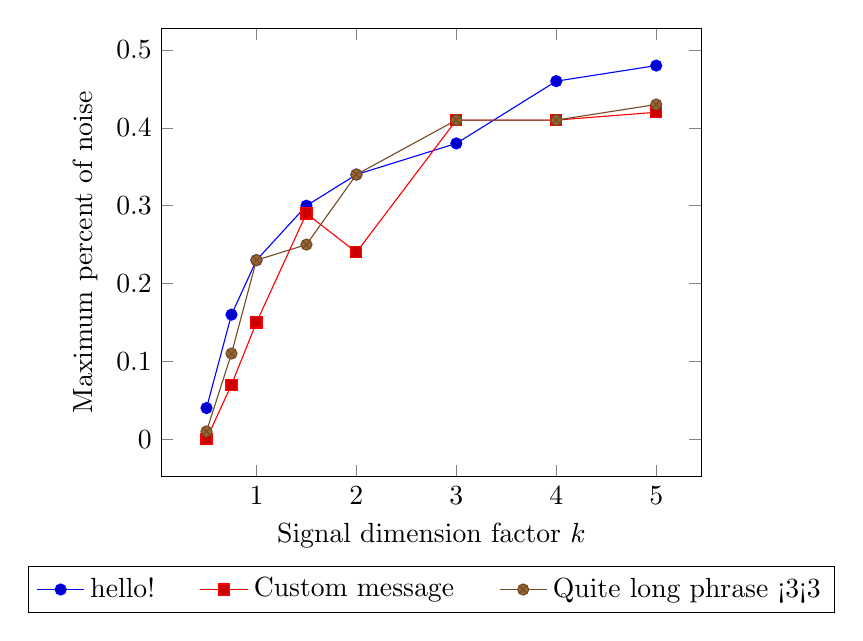
\begin{tikzpicture}
    \begin{axis}[
        legend style={at={(0.5,-0.2)},
            anchor=north,legend columns=-1},
        xlabel = Signal dimension factor $k$,
        ylabel = Maximum percent of noise,
        legend style={/tikz/every even column/.append style={column sep=0.5cm}}]
      \addplot+[sharp plot] coordinates
        {(0.5, 0.04) (0.75, 0.16) (1, 0.23) (1.5, 0.3) (2, 0.34) (3, 0.38) (4, 0.46) (5, 0.48)};

      \addplot+[sharp plot] coordinates
        {(0.5, 0.0) (0.75, 0.07) (1, 0.15) (1.5, 0.29) (2, 0.24) (3, 0.41) (4, 0.41) (5, 0.42)};

      \addplot+[sharp plot] coordinates
        {(0.5, 0.01) (0.75, 0.11) (1, 0.23) (1.5, 0.25) (2, 0.34) (3, 0.41) (4, 0.41) (5, 0.43)};

      \legend{hello!,Custom message,Quite long phrase <3<3}
    \end{axis}
  \end{tikzpicture}
  \caption[Maximum level of noise up to what the messages can be decrypted]
  {Maximum level of noise up to what the messages can be decrypted.
    Signal dimension factor $k$ is defined from equation $m=kp$ for encoding matrix $A \in \R^{m \times p}$}\label{fig:noise}
\end{figure}

\section{Q6: Dikin's method}
\ldots

\section{Q7: Integer programming}
Imposing binary (integer) variables SciPy is done via adding parameter \textit{integrality} to function \textit{scipy.optimize.linprog}. Specifically, \textit{integrality} determines for each variable whether it is integer or continuous: 0 means that parameter is continuous, 1 --- integer.

Let us for this section consider LOP in geometric form (\Cref{eq:geom}), as it is solved faster than LOP in standard form. So the integrality for $z'$ would be $w = \irow{1_p & 0_m}$, as only part of $z'$ denoting the $x$ should be restricted to be integers. Moreover, first two `row blocks' of $A'$ can be removed, and instead the \textit{bounds} parameter of \textit{scipy.optimize.linprog} can be used. The bounds would be $(0,1)$ for first $p$ coordinates of $z'$ (as $0 \leq x \leq 1$) and $(0, +\inf)$ for the last m coordinates (as $z \geq 0$). The resulting function is demonstrated on \Cref{lst:int}.

\begin{minipage}{\linewidth}
  \begin{lstlisting}[language=Python, caption={Message decryption based on solution of integer LOP in geometric form. The output is tuple of solution of the problem, and decrypted message itself}, label={lst:int}]
  def extract_message_integer(encoding_matrix, noisy_signal):

      (m, p) = encoding_matrix.shape

      c = np.zeros(p+m)
      c[p : p + m] = np.ones(m)

      integrality = np.ones(p+m) - c
      bounds = [*[(0,1) for _ in range(p)], *[(0,None) for _ in range(m)]]

      b = np.concat([ -noisy_signal, noisy_signal])

      A = np.concat(
          [
              np.concat(
                  [-encoding_matrix, np.identity(m)],
                  axis=1,
              ),
              np.concat(
                  [
                      encoding_matrix,
                      np.identity(m),
                  ],
                  axis=1,
              ),
          ]
      )

      # We add minuses, because from scipy documentation
      # A_ub x <= b_ub
      # But in geometric from we have constraints
      # A_ub x >= b_ub
      res = scipy.optimize.linprog(c, A_ub=-A, b_ub=-b,
                                   method="highs", integrality=integrality, bounds=bounds)

      return res.x, res.x[:p]
\end{lstlisting}
\end{minipage}


The results (\Cref{fig:noise_int}) show, that introducing integer restrictions increases the maximum percent of noise up to what the messages can be decrypted. However, time complexity of optimization problem with integer constraints is \textbf{significantly higher} (up to 10 times) than without integer constraints.


\begin{figure}[hbt]
  \centering
  \pgfplotsset{compat=1.10}
  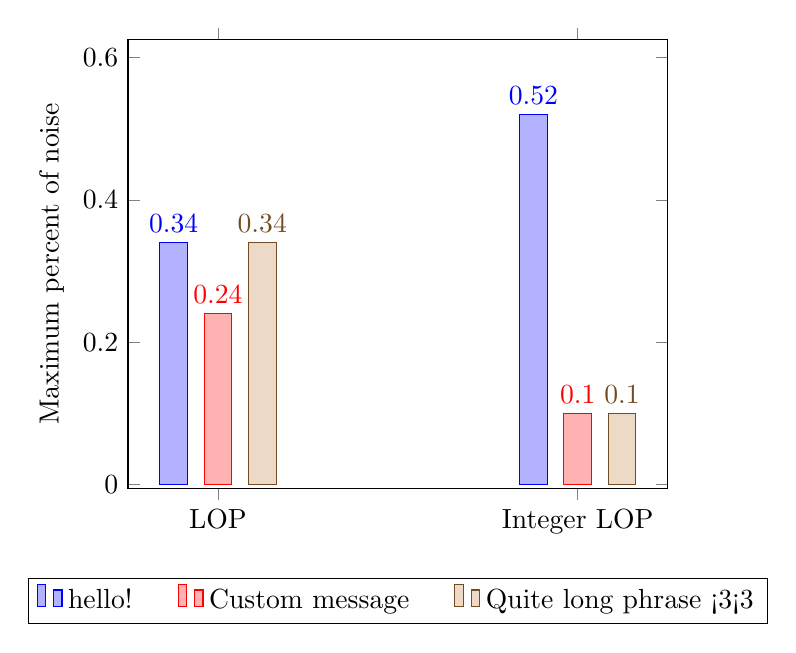
\begin{tikzpicture}
    \begin{axis}[
        ybar,
        enlargelimits=0.25,
        legend style={at={(0.5,-0.2)},
            anchor=north,legend columns=-1},
        ylabel = Maximum percent of noise,
        ybar=6pt,
        symbolic x coords={LOP,Integer LOP},
        xtick=data,
        nodes near coords,
        nodes near coords align={vertical},
        legend style={/tikz/every even column/.append style={column sep=0.5cm}}]
      \addplot coordinates {(LOP, 0.34) (Integer LOP, 0.52)};
      \addplot coordinates {(LOP, 0.24) (Integer LOP, 0.1)};
      \addplot coordinates {(LOP, 0.34) (Integer LOP, 0.1)};

      \legend{hello!,Custom message,Quite long phrase <3<3}
    \end{axis}
  \end{tikzpicture}
  \caption[Maximum level of noise up to what the messages can be decrypted (signal dimension factor $k=2$)]
  {Maximum level of noise up to what the messages can be decrypted (signal dimension factor $k=2$).
    \textit{LOP} means that no integer constraints were applied to the parameters vector, and  \textit{Integer LOP} means that integer programming was applied}\label{fig:noise_int}
\end{figure}


\end{document}
